\documentclass{beamer}

\usepackage{etoolbox}
\usepackage{graphicx}
\usepackage{enumerate}
\usepackage{verbatim}
\usepackage{tikz}
\newcommand{\HAT}[1]{\expandafter\hat#1}

\usetheme{Frankfurt}%
\usecolortheme{beaver}
%\logo{
\includegraphics[height=.125in]{img/ugaLogo}}

% %%%%%%%%%%%%%%%%%%%%%%%%%%%%%%%%%%%%%%%%%%%%%%%%%%%%%%%%%%%%%%%%%%%%%%%
% List of definitions that are used in the different pages for the
% notes

% %%%%%%%%%%%%%%%%%%%%%%%%%%%%%%%%%%%%%%%%%%%%%%%%%%%%%%%%%%%%%%%%%%%%%%%
% Basic definitions used throughout the notes

\newcommand{\half}{\mbox{$\frac{1}{2}$}}
\newcommand{\deltat}{\mbox{$\triangle t$}}
\newcommand{\deltax}{\mbox{$\triangle x$}}
\newcommand{\deltay}{\mbox{$\triangle y$}}

\newcommand{\deriv}[2]{\frac{d}{d#2}#1}
\newcommand{\derivTwo}[2]{\frac{d^2}{d#2^2}#1}

\newcommand{\lp}{\left(}
\newcommand{\rp}{\right)}


% %%%%%%%%%%%%%%%%%%%%%%%%%%%%%%%%%%%%%%%%%%%%%%%%%%%%%%%%%%%%%%%%%%%%%%
% Basic color additions
\definecolor{fuchsia}{RGB}{255,0.0,255}
\definecolor{georgiaRed}{RGB}{100,0,00}
\definecolor{light-gray}{gray}{0.8}
\definecolor{mediumGray}{gray}{0.6}


\newcommand{\redText}[1]{{\color{red}#1}}
\newcommand{\blueText}[1]{{\color{blue}#1}}
\newcommand{\greenText}[1]{{\color{green}#1}}
\newcommand{\fuchsiaText}[1]{{\color{fuchsia}#1}}


%%% Local Variables:
%%% mode: latex
%%% TeX-master: "Presentation1"
%%% End:


%\usebackgroundtemplate{
%
\includegraphics[width=\paperwidth,
%height=\paperheight]{blue.jpg}
%}

\setbeamercolor{palette primary}{fg=georgiaRed,bg=white}
\setbeamercolor{palette secondary}{fg=georgiaRed,bg=white}
\setbeamercolor{palette tertiary}{fg=georgiaRed,bg=white}
\setbeamercolor{palette quaternary}{bg=mediumGray,fg=black}
\setbeamercolor{block title}{fg=black,bg=black!15}
\setbeamercolor{block body}{fg=black,bg=black!10}
\setbeamercolor{titlelike}{bg=georgiaRed,fg=white} % parent=palette quaternary}


\setbeamercolor{upper separation line head}{bg=red}
\setbeamercolor{headline}{bg=red}
\setbeamertemplate{headline}
{
\insertsectionnavigationhorizontal{.75\textwidth}{}{}
\hfill \insertpagenumber /\insertdocumentendpage
\end{beamercolorbox}
}
%\begin{center}\begin{flushleft}\end{flushleft}\end{center}
\setbeamercolor{section number projected}{bg=red,fg=black}
\setbeamercolor{subsection number projected}{bg=red,fg=black}
\setbeamercolor{frametitle}{bg=lightgray,fg=black}


\bibliographystyle{apalike}

\begin{document}

\author{Valerie A. Carrasquillo, Claudia L. Guerrero, Michael M. Law, and Kyle McGrath}
\institute{Universidad Metropolitana, Universidad Aut\'{o}noma del Estado de Hidalgo, University of Florida, and
  SUNY-Potsdam}

\title{A Random Walk in Potsdam}
\subtitle{Adventures In Stochastic Differential Equations}
\date{June 12, 2015.}

\begin{frame}
  \titlepage
\end{frame}

\begin{frame}
  \frametitle{Outline}
  \tableofcontents
\end{frame}


\section{Biological background}

\begin{frame}
\frametitle{Coral Reef}
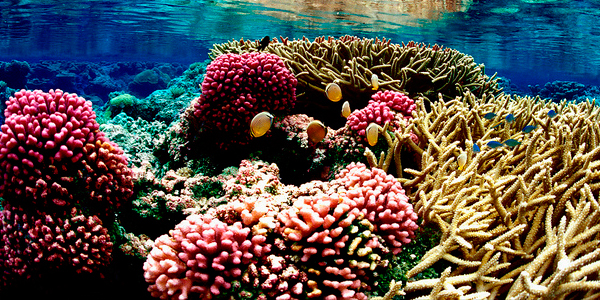
\includegraphics[scale=.175]{./US-Wildlife-coral-1.jpg}
\begin{itemize}
\item A complex aquatic ecosystem physically supported by calcium carbonate secretions of the colorful stone coral.
\item Modeling approach by Li-Wang-Zhang-Hastings is to describe the relationships between macroalgae, algal turfs, and corals (Li et al., 2014).
\end{itemize}
\end{frame}

\begin{frame}
\frametitle{Positives}
\begin{itemize}
\item Macroalgae naturally filter the water by reducing the levels of phosphate and nitrogenous waste.
\item Macroalgae provide hiding places for fishes and invertebrates
\item Macroalgae convert energy into food for the rest of the reef food web
\end{itemize}
\end{frame}

\begin{frame}
\frametitle{Coral Reef Ecosystem} 

McClanahan (1994) identifies three major components:
\begin{itemize}
\item Primary producers (coral and algae)\\
\item Herbivores (e.g. scarid grazing)\\
\item Carnivores
\end{itemize}
\end{frame}

\begin{frame}
\centering
\frametitle{Reef Food Web}
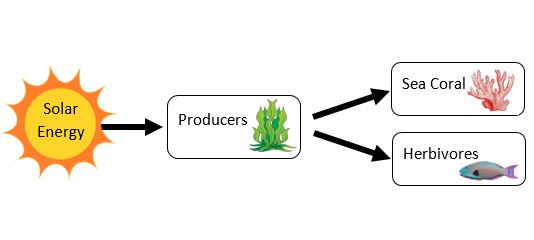
\includegraphics[scale=.65]{./CoralFoodWeb}
\end{frame}

\begin{frame}
\frametitle{Negatives}
\begin{itemize}
\item At low grazing levels, the macroalgal population increases and competes with the coral population for space.
\item This competition alters the microbial communities associated with corals increasing pathogens on corals.
\item Macroalgal abundance may lead to reef degradation.
\item Coral mortality is generally followed by algal recruitment.
\end{itemize}
\end{frame}

\begin{frame}
\frametitle{Coral Reef Dynamics}
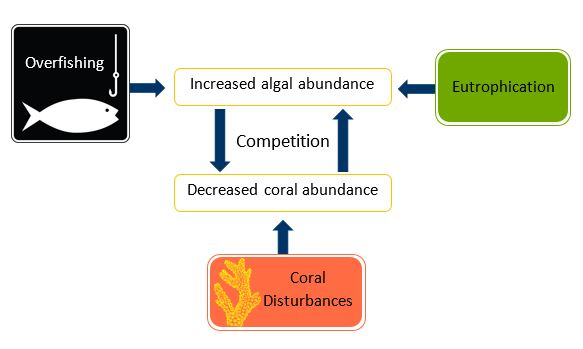
\includegraphics[scale=.7]{./CoralDynamics}
\end{frame}


\section{Modeling Coral Reef Dynamics}

\begin{frame}
\frametitle{Coral Reef Dynamics}
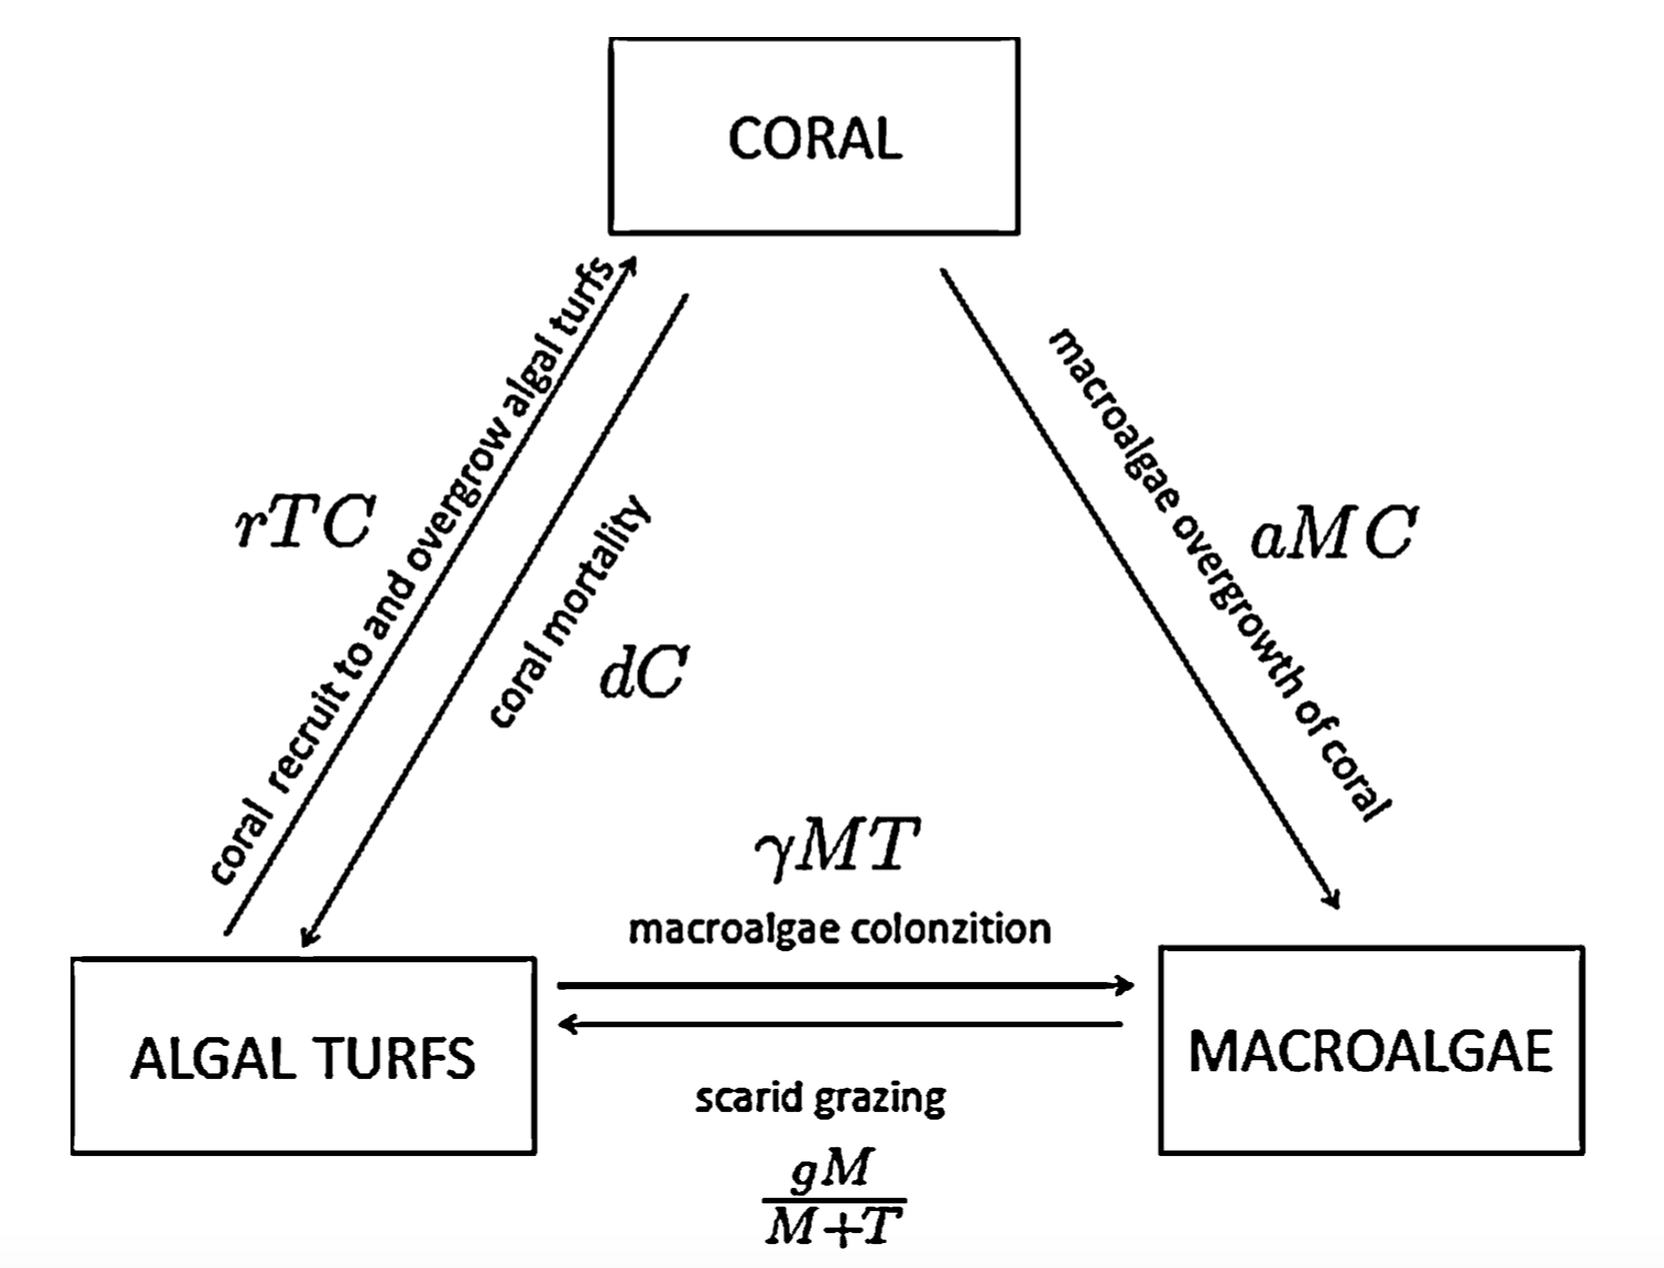
\includegraphics[scale=.175]{./coral-reef-triangle.png}
\end{frame}

\begin{frame}\frametitle{Coral Reef Dynamics}
The deterministic ordinary differential equation model:
$$\begin{cases}\begin{array}{rl}
\frac{dM}{dt}\hspace{-.8em}&=aMC - \frac{gM}{M+T} + \gamma M T, \\
\frac{dC}{dt}\hspace{-.8em}&=rTC - dC - aMC, \\
\frac{dT}{dt}\hspace{-.8em}&=\frac{gM}{M + T} - \gamma MT - rTC + dC. 
\end{array}\end{cases}$$ 

where 
\begin{itemize}\itemsep0pt
\item $r$ is the rate corals overgrow upon algal turfs\\
\item $d$ is the mortality rate of corals\\
\item $a$ is the rate that macroalgae overgrow upon corals\\
\item $\gamma$ is the rate that macroalgae spread over algal turfs\\
\item $g$ is the indiscriminate grazing rate of parrotfish.
\end{itemize}
\end{frame}

\begin{frame}\frametitle{Coral Reef Dynamics}

\hspace{1.57em}

\begin{itemize}
\item $\frac{dT}{dt}=-\frac{dM}{dt}-\frac{dC}{dt}$ implies $M+C+T$ is
  constant.
\item We assume that $M+C+T=1$.
\item This limits our scope to regions entirely covered by coral,
  macroalgae, and algal turf. 
\end{itemize}

Thus, we reduce our system to, 
$$\begin{cases}
\begin{array}{rl}
\frac{dM}{dt}&= aMC-\frac{gM}{1-C} + \gamma M - \gamma M^2 -\gamma M C,\\
\frac{dC}{dt}&=rC - rC^2 - rCM - dC - aMC.
\end{array} 
\end{cases}$$
\end{frame}


\begin{comment}\frametitle{Equilibria and Stability}
Equilibrium point

\end{comment}

\begin{frame}\frametitle{Equilibria and Stability}
To find equilibrium points analytically we first set the derivatives equal to zero to obtain the nullclines:
$$\begin{cases}
\begin{array}{rl}
0\hspace{-.8em}&=M(aC + \gamma-\gamma M-\gamma C) - \frac{gM}{1-C},\\
0\hspace{-.8em}&=C(r-Mr-Cr - d - aM).\\
\end{array}
\end{cases}$$
\end{frame}

\begin{frame}\frametitle{Equilibria and Stability}\begin{itemize}
\item $M'=0$ is satisfied when:\begin{itemize}\item $M=0$, or \item $aC + \gamma - \gamma M - \gamma C - \frac{gM}{1-C}=0$.\end{itemize}
\item $C'=0$ is satisfied when:\begin{itemize} \item$C=0$, or \item $r-Mr-Cr-d-aM=0$. \end{itemize}
\end{itemize}
\end{frame}

\begin{frame}\frametitle{Phase Plane} Our equilibrium points are located at the intersections of the nullclines:
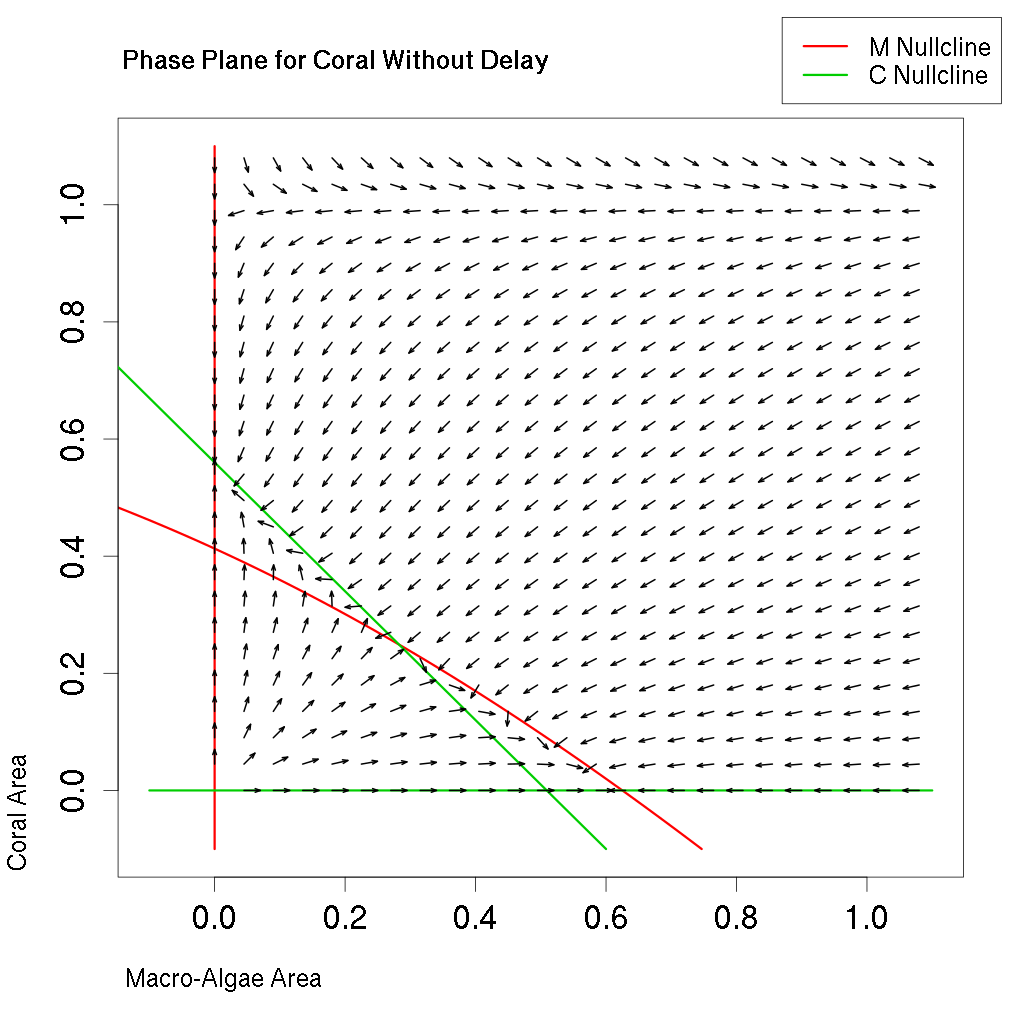
\includegraphics[scale=.22]{./nullclines.png}
\end{frame}

\begin{frame}
\frametitle{Time Delay in the Coral Ecosystem}
We can identify time delays in the coral ecosystem:
\begin{itemize}
\item the delay between overfishing of herbivores and growth of macroalgae.\\
\item the delay between the growth of algae and the effect of algae on coral (Jompa, 2003).\\
\item the delay between the grazing of macroalgae and growth of algal turf (Li et al., 2014).
\end{itemize} We focus on the third time delay.
\end{frame}

\begin{frame}\frametitle{Coral Reef Dynamics}
Delay Differential Equation Model:
$$\begin{cases}
\begin{array}{rl}
\frac{dM}{dt}\hspace{-.8em}&=aMC - \frac{gM(t-\tau)}{1-C(t-\tau)} + \gamma M (1-M-C),\\
\frac{dC}{dt}\hspace{-.8em}&=rC(1-M-C) - dC - aMC,\\
\end{array}
\end{cases}$$ where $\tau$ is our time delay.
\end{frame}

\begin{frame}
\frametitle{Equilibria and Stability}
There are three equilibrium points of interest: \begin{itemize}
\item $(0,0)$ (Unstable for all $\tau\geq0$)\\
\item $(1-\frac{g}{\gamma},0)$ (High Coral Cover)\\
\item $(0,1-\frac{d}{r})$ (High Algae Cover).
\end{itemize} Notice that time delay does not affect the equilibria.
\end{frame}

\begin{frame}\frametitle{Jacobian Matrices}
We linearize our delay model:{\small $\begin{bmatrix} M'\\C'\end{bmatrix}=J_1\begin{bmatrix} M\\C\end{bmatrix}+J_2\begin{bmatrix}M(t-\tau)\\C(t-\tau)\end{bmatrix}$ (call this eq'n 1), where $$J_1=\begin{bmatrix}\gamma-2\gamma M +(a-\gamma)C & (a-\gamma)M\\ -(a+r)C & r-d-(a+r)-2MC \end{bmatrix}, \text{ and}$$ $$J_2=\begin{bmatrix} \frac{-g}{1-C(t-\tau)} & \frac{-gM(t-\tau)}{(1-C(t-\tau))^2}\\ 0 & 0\end{bmatrix}.$$}
\end{frame}

\begin{comment}

\begin{frame}\frametitle{Putting Jacobians to Use}
{ Suppose $\begin{bmatrix} x\\y\end{bmatrix}=\overrightarrow{v_1}e^{\lambda t}$.}\\\vspace{2em} 
{ Differentiating, setting equal to 1, and doing algebra stuff, we get $(J_1+J_2e^{-\lambda t} -\lambda I)\overrightarrow{v_1}=0$.} 
\end{frame}
\end{comment}

\begin{frame}\frametitle{Putting Jacobians to Use}
Consider the Jacobians evaluated at the origin:$$J_1=\begin{bmatrix}
\gamma & 0\\
0 & r-d
\end{bmatrix}, \text{ and}$$ $$J_2=\begin{bmatrix}
-g & 0\\
0 & 0
\end{bmatrix}.$$ 
\end{frame}


\begin{frame}[c]\frametitle{Putting Jacobians to Use}
%Recall, $(J_1+J_2e^{-\lambda t} -\lambda I)\overrightarrow{v_1}=0$. \\\vspace{2em} Taking determinants, we find the characteristic polynomial of $(J_1+J_2e^{-\lambda t} -\lambda I)$ evaluated at $M=0$, $C=0$ to be 
The characteristic polynomial of $$(J_1+J_2e^{-\lambda t} -\lambda I),\text{ is}$$ $$(\lambda - r + d)(\lambda -\gamma + ge^{-\lambda\tau})=0$$. 
\end{frame}

\begin{frame}\frametitle{Get Them Eigenvalues}
Hence, \begin{itemize}{\itemsep .5in}\item $\lambda = r-d>0$ is an eigenvalue with positive real part\item Other eigenvalues satisfy $\lambda=\gamma-ge^{-\lambda\tau}$. \item For $\tau\geq0$, our system has two eigenvalues with positive real part. This implies our nondelay system is unstable at $(0,0)$. \end{itemize}\end{frame}

\begin{comment}
\begin{frame}\frametitle{Get Them Eigenvalues}
Now we consider postive $\tau$.
\begin{itemize}
\item Let $\lambda \tau=(\alpha+i\omega)\tau$.
\item Apply Euler's Formula: $\gamma-g(e^{-\lambda\tau})=\gamma-g(\cos(\lambda\tau)-i\sin(\lambda\tau))$.
\end{itemize}
\end{frame}\end{comment}

\begin{frame}
The time delay model fails to account for stochastic features of the ecosystem:
\begin{itemize}
\item grazing habits of parrotfish, and;
\item hurricanes.
\end{itemize}
\end{frame}

\begin{frame}
\frametitle{Stochastic Model}
To account for these stochastic feature we add noise!
$$\begin{cases}
\begin{array}{rl}
\frac{dM}{dt}\hspace{-.8em}&=aMC - \frac{gM(t-\tau)}{1-C(t-\tau)}+\gamma M T+\beta M(1-M)dW,\\
\frac{dC}{dt}\hspace{-.8em}&=rTC - dC - aMC.\\
\end{array}
\end{cases}$$
\end{frame}

\begin{frame}

\end{frame}
\section{Conclusions}

\begin{frame}
  \frametitle{Conclusions}

  A bunch of stuff goes here.

\end{frame}

\begin{frame}
  \frametitle{title}
  
\end{frame}

\begin{frame}
  \frametitle{Bibliography}
  
\end{frame}

\begin{frame}
  \frametitle{Acknowledgments}
  
  We would like to thank the following for their support and funding: 
  
 \begin{itemize}
 \item Dr. Joel Foisy, SUNY Potsdam
 \item National Security Agency (H98230-14-1-0141)
 \item National Science Foundation (DSM-1262737)
 \end{itemize}
\end{frame}



%%% Local Variables:
%%% mode: latex
%%% TeX-master: "Presentation1"
%%% End:

\end{document}
